% JUNA grant-body slide deck
% Compile with: pdflatex juna_grant_body_slides.tex
\documentclass[aspectratio=169,10pt]{beamer}

\usepackage[T1]{fontenc}
\usepackage{amsmath,amssymb}
\usepackage{booktabs}
\usepackage{graphicx}
\usepackage{tikz}
\usepackage{xcolor}
\usetikzlibrary{arrows.meta,positioning,calc,fit,shapes.geometric,decorations.pathmorphing}

\definecolor{bg}{HTML}{F7F3EA}
\definecolor{panel}{HTML}{FFFCF5}
\definecolor{text}{HTML}{1D2528}
\definecolor{muted}{HTML}{657074}
\definecolor{juna}{HTML}{23684A}
\definecolor{rpc}{HTML}{A43B36}
\definecolor{pilot}{HTML}{2D6CDF}
\definecolor{data}{HTML}{6E7378}
\definecolor{nullc}{HTML}{ECE5D8}
\definecolor{gold}{HTML}{C08A2D}
\definecolor{grid}{HTML}{CFC7B7}
\definecolor{accent}{HTML}{0F4C81}

\usefonttheme{professionalfonts}
\setbeamercolor{background canvas}{bg=bg}
\setbeamercolor{normal text}{fg=text}
\setbeamercolor{frametitle}{fg=text,bg=bg}
\setbeamercolor{structure}{fg=juna}
\setbeamercolor{calloutbox}{fg=text,bg=panel}
\setbeamertemplate{navigation symbols}{}
\setbeamertemplate{itemize item}{\raise0.15ex\hbox{\scriptsize$\blacktriangleright$}}
\setbeamerfont{frametitle}{series=\bfseries,size=\Large}
\setbeamertemplate{frametitle}{%
  \vspace{0.25em}
  \insertframetitle\par
  \vspace{0.25em}
  {\color{grid}\rule{0.94\paperwidth}{0.5pt}}
}
\setbeamertemplate{footline}{%
  \hfill{\scriptsize\color{muted}JUNA \textendash{} Doppler-resilient underwater OFDM\quad\insertframenumber}\hspace{0.5cm}\vspace{0.25cm}
}

\newcommand{\metric}[2]{\textbf{#1:} #2}
\newcommand{\channelimage}[1]{\includegraphics[width=\linewidth,height=0.40\paperheight,keepaspectratio]{#1}}
\newenvironment{callout}{%
  \begin{beamercolorbox}[wd=\linewidth,sep=4pt,rounded=true]{calloutbox}\scriptsize%
}{%
  \end{beamercolorbox}%
}

\tikzset{
  block/.style={draw=text, fill=panel, rounded corners=2pt, line width=0.55pt,
                align=center, inner sep=5pt, font=\small},
  arrow/.style={-{Stealth[length=2.4mm]}, line width=0.7pt, draw=text},
  callout/.style={draw=grid, fill=panel, rounded corners=2pt, line width=0.45pt,
                  align=left, inner sep=6pt, font=\small},
  tinycell/.style={draw=grid, line width=0.25pt, minimum width=0.33cm,
                   minimum height=0.33cm, inner sep=0pt}
}

\begin{document}

% =====================================================================
% 1. TITLE PAGE WITH ARL LOGO
% =====================================================================
\begin{frame}[plain]
  \vspace{0.4cm}
  \begin{center}
    \includegraphics[height=3.2cm,keepaspectratio]{arllogo.png}\\[0.5cm]
    {\Huge\bfseries\color{accent} JUNA\par}
    \vspace{0.25cm}
    {\Large A joint receiver--decoder for\\
     \textbf{Doppler-resilient underwater communication}\par}
    \vspace{0.9cm}
    {\large First milestone review\par}
    \vspace{0.2cm}
    {\color{muted}\small Acoustic Research Laboratory}
  \end{center}
\end{frame}

% 3. PLAIN-LANGUAGE EXPLANATION OF THE PROBLEM (short)
% =====================================================================
\begin{frame}{The problem, in plain terms}
  \vspace{-0.15cm}
  {\footnotesize OFDM sends many \emph{tones} simultaneously \textendash{} each tone carries one BPSK bit ($\pm 1$); $N$ tones $\to$ $N$ coded bits per OFDM symbol.}
  \vspace{0.05cm}

  % --- Compact bit-to-tone mapping diagram ---
  \centering
  \resizebox{0.78\linewidth}{!}{%
  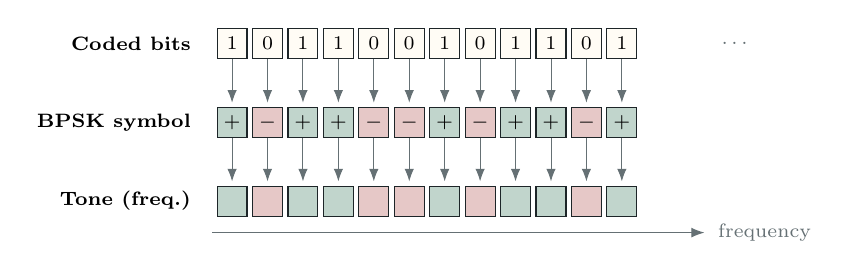
\begin{tikzpicture}[x=1cm,y=1cm,>=Latex,font=\scriptsize]
    \node[font=\scriptsize\bfseries,anchor=east] at (1.0,3.0) {Coded bits};
    \foreach \i/\b in {0/1,1/0,2/1,3/1,4/0,5/0,6/1,7/0,8/1,9/1,10/0,11/1} {
      \pgfmathsetmacro{\xx}{1.4+\i*0.45}
      \node[draw=text,fill=panel,minimum size=0.38cm,inner sep=0pt] at (\xx,3.0) {\b};
    }
    \node[anchor=west,text=muted] at (7.4,3.0) {\,\,\dots};

    \node[font=\scriptsize\bfseries,anchor=east] at (1.0,2.0) {BPSK symbol};
    \foreach \i/\v/\col in {0/$+$/juna,1/$-$/rpc,2/$+$/juna,3/$+$/juna,4/$-$/rpc,5/$-$/rpc,6/$+$/juna,7/$-$/rpc,8/$+$/juna,9/$+$/juna,10/$-$/rpc,11/$+$/juna} {
      \pgfmathsetmacro{\xx}{1.4+\i*0.45}
      \draw[->,draw=muted,line width=0.35pt] (\xx,2.80) -- (\xx,2.25);
      \node[draw=text,fill=\col!28,minimum size=0.38cm,inner sep=0pt] at (\xx,2.0) {\v};
    }

    \node[font=\scriptsize\bfseries,anchor=east] at (1.0,1.0) {Tone (freq.)};
    \foreach \i/\col in {0/juna,1/rpc,2/juna,3/juna,4/rpc,5/rpc,6/juna,7/rpc,8/juna,9/juna,10/rpc,11/juna} {
      \pgfmathsetmacro{\xx}{1.4+\i*0.45}
      \draw[->,draw=muted,line width=0.35pt] (\xx,1.80) -- (\xx,1.25);
      \node[draw=text,fill=\col!28,minimum size=0.38cm,inner sep=0pt] at (\xx,1.0) {};
    }
    \draw[->,draw=muted] (1.15,0.6) -- (7.4,0.6);
    \node[font=\scriptsize,text=muted,anchor=west] at (7.45,0.6) {frequency};
  \end{tikzpicture}}
  \vspace{0.05cm}

  % --- Bottom row: text + waveforms ---
  \begin{columns}[T,onlytextwidth]
    \begin{column}{0.40\textwidth}
      \scriptsize\textbf{Still channel.} Each tone arrives on its own frequency \textendash{} mapping preserved.
      \vspace{0.3em}

      \scriptsize\textbf{Motion / Doppler.} Tones drift off frequency, neighbours overlap, mapping breaks.
    \end{column}
    \begin{column}{0.58\textwidth}
      \resizebox{\linewidth}{!}{%
      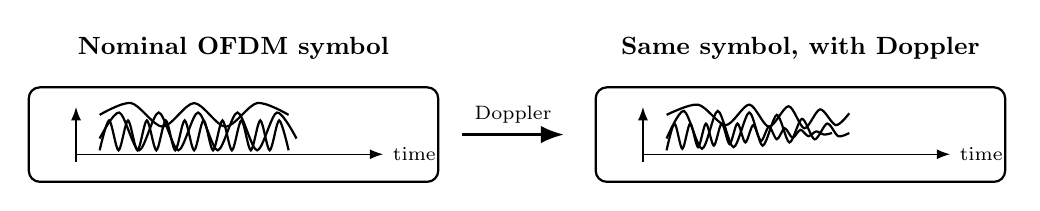
\begin{tikzpicture}[x=1cm,y=1cm,>=Latex]
        \node[font=\small\bfseries] at (3.0,5.8) {Nominal OFDM symbol};
        \draw[rounded corners, thick] (0.4,4.1) rectangle (5.6,5.3);
        \draw[->] (1.0,4.45) -- (4.9,4.45) node[right] {\scriptsize time};
        \draw[->] (1.0,4.35) -- (1.0,5.05);
        \draw[thick] plot[smooth] coordinates {(1.3,4.95) (1.7,5.10) (2.1,4.80) (2.5,5.10) (2.9,4.80) (3.3,5.10) (3.7,4.95)};
        \draw[thick] plot[smooth] coordinates {(1.3,4.65) (1.55,4.98) (1.8,4.50) (2.05,4.98) (2.30,4.50) (2.55,4.98) (2.80,4.50) (3.05,4.98) (3.30,4.50) (3.55,4.98) (3.80,4.65)};
        \draw[thick] plot[smooth] coordinates {(1.3,4.50) (1.42,4.88) (1.54,4.50) (1.66,4.88) (1.78,4.50) (1.90,4.88) (2.02,4.50) (2.14,4.88) (2.26,4.50) (2.38,4.88) (2.50,4.50) (2.62,4.88) (2.74,4.50) (2.86,4.88) (2.98,4.50) (3.10,4.88) (3.22,4.50) (3.34,4.88) (3.46,4.50) (3.58,4.88) (3.70,4.50)};

        \node[font=\small\bfseries] at (10.2,5.8) {Same symbol, with Doppler};
        \draw[rounded corners, thick] (7.6,4.1) rectangle (12.8,5.3);
        \draw[->] (8.2,4.45) -- (12.1,4.45) node[right] {\scriptsize time};
        \draw[->] (8.2,4.35) -- (8.2,5.05);
        \draw[thick] plot[smooth] coordinates {(8.5,4.95) (8.9,5.08) (9.25,4.82) (9.55,5.08) (9.80,4.80) (10.05,5.06) (10.25,4.78) (10.45,5.02) (10.65,4.82) (10.82,4.97)};
        \draw[thick] plot[smooth] coordinates {(8.5,4.65) (8.72,5.00) (8.95,4.52) (9.15,5.00) (9.35,4.54) (9.55,4.98) (9.72,4.56) (9.90,4.95) (10.06,4.60) (10.22,4.90) (10.38,4.64) (10.54,4.84) (10.68,4.68) (10.82,4.72)};
        \draw[thick] plot[smooth] coordinates {(8.5,4.50) (8.60,4.84) (8.70,4.52) (8.80,4.84) (8.90,4.54) (9.00,4.84) (9.10,4.56) (9.20,4.84) (9.30,4.58) (9.40,4.84) (9.50,4.60) (9.60,4.82) (9.70,4.62) (9.80,4.80) (9.90,4.64) (10.00,4.78) (10.10,4.66) (10.20,4.76) (10.30,4.68) (10.40,4.74) (10.50,4.70) (10.60,4.72)};

        \draw[very thick,->] (5.9,4.7) -- (7.2,4.7);
        \node[font=\scriptsize] at (6.55,4.95) {Doppler};
      \end{tikzpicture}}
    \end{column}
  \end{columns}
\end{frame}

% =====================================================================
% 2. ONE-MINUTE PITCH
% =====================================================================
\begin{frame}{Where we are, in one minute}
  \vspace{0.1cm}
  \begin{columns}[T,onlytextwidth]
    \begin{column}{0.32\textwidth}
      \begin{beamercolorbox}[wd=\linewidth,sep=6pt,rounded=true]{calloutbox}
        \textbf{\color{rpc} The problem}\\[0.2em]
        \scriptsize Doppler (motion) breaks subcarrier orthogonality \textendash{} energy leaks between carriers (ICI).
      \end{beamercolorbox}
    \end{column}
    \begin{column}{0.32\textwidth}
      \begin{beamercolorbox}[wd=\linewidth,sep=6pt,rounded=true]{calloutbox}
        \textbf{\color{accent} State of the art}\\[0.2em]
        \scriptsize \textbf{RPC} \textendash{} a recursive partial-FFT combiner \textendash{} corrects the phase/weighting and recovers symbols under Doppler. \emph{Combiner weights are learned from pilots} \textendash{} so it is pilot-hungry.
      \end{beamercolorbox}
    \end{column}
    \begin{column}{0.32\textwidth}
      \begin{beamercolorbox}[wd=\linewidth,sep=6pt,rounded=true]{calloutbox}
        \textbf{\color{juna} What JUNA does}\\[0.2em]
        \scriptsize Combiner weights, soft symbols, and LDPC decoding are trained in a \textbf{single joint learning process} \textendash{} the code shares the load. \textbf{Fewer pilots} at the same reliability \textendash{} so \textbf{higher data rate}.
      \end{beamercolorbox}
    \end{column}
  \end{columns}

  \vspace{0.20cm}
  \begin{center}
  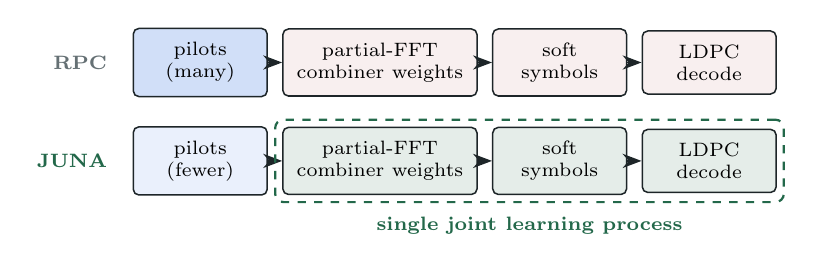
\begin{tikzpicture}[node distance=0.18cm,font=\scriptsize]
    % RPC row
    \node[block,minimum width=1.7cm,minimum height=0.55cm,font=\scriptsize,fill=pilot!22] (rp1) {pilots\\(many)};
    \node[block,minimum width=2.4cm,minimum height=0.55cm,font=\scriptsize,right=of rp1,fill=rpc!8] (rp2) {partial-FFT\\combiner weights};
    \node[block,minimum width=1.7cm,minimum height=0.55cm,font=\scriptsize,right=of rp2,fill=rpc!8] (rp3) {soft\\symbols};
    \node[block,minimum width=1.7cm,minimum height=0.55cm,font=\scriptsize,right=of rp3,fill=rpc!8] (rp4) {LDPC\\decode};
    \draw[arrow] (rp1) -- (rp2);
    \draw[arrow] (rp2) -- (rp3);
    \draw[arrow] (rp3) -- (rp4);
    \node[font=\scriptsize,text=muted,left=0.20cm of rp1] {\textbf{RPC}};

    % JUNA row
    \begin{scope}[yshift=-1.25cm]
      \node[block,minimum width=1.7cm,minimum height=0.55cm,font=\scriptsize,fill=pilot!10] (jp1) {pilots\\(fewer)};
      \node[block,minimum width=2.4cm,minimum height=0.55cm,font=\scriptsize,right=of jp1,fill=juna!12] (jp2) {partial-FFT\\combiner weights};
      \node[block,minimum width=1.7cm,minimum height=0.55cm,font=\scriptsize,right=of jp2,fill=juna!12] (jp3) {soft\\symbols};
      \node[block,minimum width=1.7cm,minimum height=0.55cm,font=\scriptsize,right=of jp3,fill=juna!12] (jp4) {LDPC\\decode};
      \draw[arrow] (jp1) -- (jp2);
      \draw[arrow] (jp2) -- (jp3);
      \draw[arrow] (jp3) -- (jp4);
      \node[draw=juna,dashed,line width=0.8pt,rounded corners=3pt,
            fit=(jp2)(jp3)(jp4),inner sep=2.5pt] (joint) {};
      \node[font=\scriptsize\bfseries,text=juna,below=0.05cm of joint.south] {single joint learning process};
      \node[font=\scriptsize,text=juna,left=0.20cm of jp1] {\textbf{JUNA}};
    \end{scope}
  \end{tikzpicture}
  \end{center}
\end{frame}

% =====================================================================
% 2b. JUNA IN CONTEXT: DFEC LINEAGE
% =====================================================================
\begin{frame}{JUNA inherits from the DFEC line of work}
  \vspace{0.4cm}
  \begin{columns}[T,onlytextwidth]
    \begin{column}{0.48\textwidth}
      \begin{beamercolorbox}[wd=\linewidth,sep=10pt,rounded=true]{calloutbox}
        \textbf{\color{accent} DFEC} \,{\scriptsize\color{muted}(prior work)}\\[0.5em]
        \small
        \textbf{Setting:} single-carrier, ISI.\\[0.35em]
        \textbf{Unknowns:} FIR taps + coded symbols.
      \end{beamercolorbox}
    \end{column}
    \begin{column}{0.48\textwidth}
      \begin{beamercolorbox}[wd=\linewidth,sep=10pt,rounded=true]{calloutbox}
        \textbf{\color{juna} JUNA} \,{\scriptsize\color{muted}(this work)}\\[0.5em]
        \small
        \textbf{Setting:} OFDM, Doppler/ICI.\\[0.35em]
        \textbf{Unknowns:} impulse response \(\to\) combiner weights + coded symbols.
      \end{beamercolorbox}
    \end{column}
  \end{columns}
  \vspace{0.6cm}
  \begin{center}
    \large\bfseries\color{accent}
    Same idea: code constraints inside symbol recovery.
  \end{center}
\end{frame}


% =====================================================================
% 4. NO DOPPLER VS DOPPLER (original slide 1)
% =====================================================================
\begin{frame}{No Doppler vs Doppler: What Changes}
  \centering
  {\small\textbf{Example scale:} a 12 kHz acoustic band split into 1000 carriers gives
  $\Delta f = 12$ Hz per carrier.}\par
  \vspace{0.05cm}
  {\scriptsize Each row/column below is one carrier position; for BPSK, one carrier symbol is one coded bit position.}\par
  \vspace{0.08cm}
  {\scriptsize
    \tikz[baseline=-0.5ex]\node[tinycell,fill=juna!70]{};\, on-diagonal\quad
    \tikz[baseline=-0.5ex]\node[tinycell,fill=gold!70]{};\, immediate-neighbour leakage\quad
    \tikz[baseline=-0.5ex]\node[tinycell,fill=rpc!45]{};\, further-neighbour leakage\quad
    \tikz[baseline=-0.5ex]\node[tinycell,fill=nullc]{};\, no coupling}\par
  \vspace{0.1cm}
  \begin{columns}[T,onlytextwidth]
    \begin{column}{0.49\textwidth}
      \centering
      \textbf{No residual Doppler}\par
      \vspace{0.12cm}
      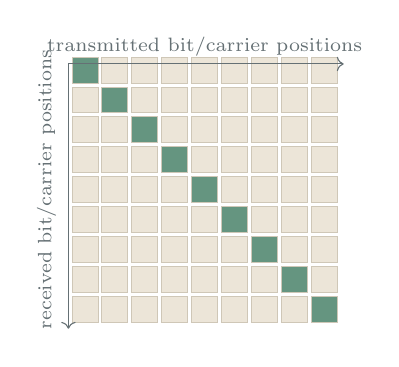
\begin{tikzpicture}[scale=0.38]
        \foreach \i in {0,...,8} {
          \foreach \j in {0,...,8} {
            \node[tinycell,fill=nullc] at (\i,-\j) {};
          }
        }
        \foreach \i in {0,...,8} {
          \node[tinycell,fill=juna!70] at (\i,-\i) {};
        }
        \draw[->,draw=muted] (-0.55,0.2) -- (8.65,0.2);
        \draw[->,draw=muted] (-0.55,0.2) -- (-0.55,-8.65);
        \node[font=\scriptsize,text=muted] at (4.0,0.78) {transmitted bit/carrier positions};
        \node[font=\scriptsize,text=muted,rotate=90] at (-1.28,-4.0) {received bit/carrier positions};
      \end{tikzpicture}
      \vspace{0.05cm}
      {\scriptsize Each received carrier mainly depends on the same transmitted carrier.}
    \end{column}
    \begin{column}{0.49\textwidth}
      \centering
      \textbf{Residual Doppler}\par
      \vspace{0.12cm}
      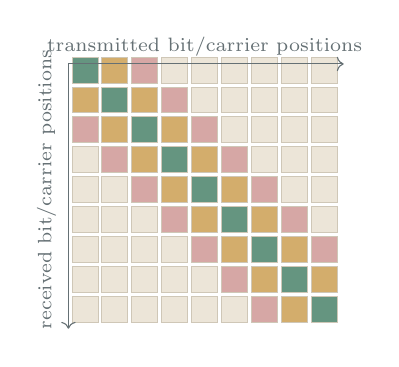
\begin{tikzpicture}[scale=0.38]
        \foreach \i in {0,...,8} {
          \foreach \j in {0,...,8} {
            \node[tinycell,fill=nullc] at (\i,-\j) {};
          }
        }
        \foreach \i in {0,...,8} {
          \node[tinycell,fill=juna!70] at (\i,-\i) {};
        }
        \foreach \i/\j in {1/0,2/1,3/2,4/3,5/4,6/5,7/6,8/7,0/1,1/2,2/3,3/4,4/5,5/6,6/7,7/8} {
          \node[tinycell,fill=gold!70] at (\i,-\j) {};
        }
        \foreach \i/\j in {2/0,3/1,4/2,5/3,6/4,7/5,8/6,0/2,1/3,2/4,3/5,4/6,5/7,6/8} {
          \node[tinycell,fill=rpc!45] at (\i,-\j) {};
        }
        \draw[->,draw=muted] (-0.55,0.2) -- (8.65,0.2);
        \draw[->,draw=muted] (-0.55,0.2) -- (-0.55,-8.65);
        \node[font=\scriptsize,text=muted] at (4.0,0.78) {transmitted bit/carrier positions};
        \node[font=\scriptsize,text=muted,rotate=90] at (-1.28,-4.0) {received bit/carrier positions};
      \end{tikzpicture}
      \vspace{0.05cm}
      {\scriptsize Energy leaks into neighboring carriers; recovery becomes a coupled problem.}
    \end{column}
  \end{columns}
\end{frame}

% =====================================================================
% 6. PILOTS AND CHANNELS (was slide 2)
% =====================================================================
\begin{frame}{How the receiver normally orients itself}
  \centering
  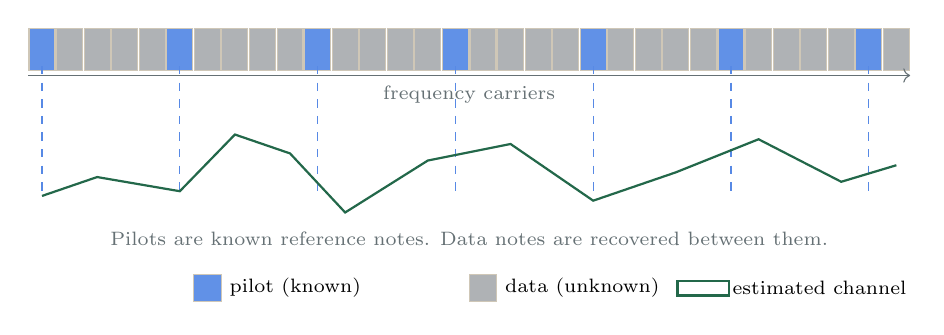
\begin{tikzpicture}[x=0.35cm,y=0.60cm]
    \foreach \i in {0,...,31} {
      \node[draw=grid,fill=data!55,minimum width=0.33cm,minimum height=0.54cm,inner sep=0pt] at (\i,0) {};
    }
    \foreach \i in {0,5,10,15,20,25,30} {
      \node[draw=grid,fill=pilot!75,minimum width=0.33cm,minimum height=0.54cm,inner sep=0pt] at (\i,0) {};
    }
    \draw[->,draw=muted] (-0.5,-0.55) -- (31.5,-0.55);
    \node[font=\scriptsize,text=muted] at (15.5,-0.95) {frequency carriers};
    \foreach \x in {0,5,10,15,20,25,30} {
      \draw[dashed,draw=pilot!80] (\x,-0.35) -- (\x,-3.1);
    }
    \draw[thick,juna] (0,-3.1) -- (2,-2.7) -- (5,-3.0) -- (7,-1.8) -- (9,-2.2)
      -- (11,-3.45) -- (14,-2.35) -- (17,-2.0) -- (20,-3.2) -- (23,-2.6)
      -- (26,-1.9) -- (29,-2.8) -- (31,-2.45);
    \node[font=\scriptsize,text=muted] at (15.5,-4.0)
      {Pilots are known reference notes. Data notes are recovered between them.};
    \node[fill=pilot!75,draw=grid,minimum width=0.35cm,minimum height=0.35cm] at (6.0,-5.05) {};
    \node[font=\scriptsize,anchor=west] at (6.45,-5.05) {pilot (known)};
    \node[fill=data!55,draw=grid,minimum width=0.35cm,minimum height=0.35cm] at (16.0,-5.05) {};
    \node[font=\scriptsize,anchor=west] at (16.45,-5.05) {data (unknown)};
    \node[draw=juna,line width=1pt,minimum width=0.65cm,minimum height=0.18cm,inner sep=0pt] at (24.0,-5.05) {};
    \node[font=\scriptsize,anchor=west] at (24.7,-5.05) {estimated channel};
  \end{tikzpicture}
  \vspace{0.25cm}
  \begin{columns}[T,onlytextwidth]
    \begin{column}{0.31\textwidth}
      \small\textbf{The channel} bends and notches the signal because of echoes off the surface and sea bed.
    \end{column}
    \begin{column}{0.31\textwidth}
      \small\textbf{Pilots} are known anchors. More anchors = better tracking, but less room for payload.
    \end{column}
    \begin{column}{0.31\textwidth}
      \small\textbf{JUNA} adds a third anchor \textendash{} the error-correcting code itself \textendash{} so fewer pilots can do the same job.
    \end{column}
  \end{columns}
\end{frame}

% =====================================================================
% 7. PARTIAL-FFT COMBINING AND JUNA
% =====================================================================
\begin{frame}{Partial-FFT combining: separating carriers that now talk to each other}
  \vspace{-0.05cm}
  {\footnotesize Under Doppler, one FFT mixes neighbouring tones. Slice the symbol in time, get several views of each tone, then combine them \textendash{} the trick is choosing the weights.}
  \vspace{0.15cm}

  \begin{columns}[T,onlytextwidth]
    % ---------- Panel 1: the problem ----------
    \begin{column}{0.30\textwidth}
      \centering
      \textbf{\small 1.\ One FFT $=$ local mixture}\par
      \vspace{0.25cm}
      \resizebox{0.95\linewidth}{!}{%
      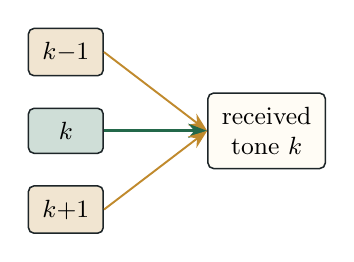
\begin{tikzpicture}[x=1cm,y=1cm,>=Latex]
        \node[block,minimum width=0.95cm,minimum height=0.55cm,fill=gold!22] (km) at (0,1.0) {\small$k{-}1$};
        \node[block,minimum width=0.95cm,minimum height=0.55cm,fill=juna!22] (k)  at (0,0.0) {\small$k$};
        \node[block,minimum width=0.95cm,minimum height=0.55cm,fill=gold!22] (kp) at (0,-1.0) {\small$k{+}1$};
        \node[block,minimum width=1.40cm,minimum height=0.75cm,fill=panel] (yk) at (2.55,0.0) {\small received\\\small tone $k$};
        \draw[arrow,draw=gold] (km.east) -- (yk.west);
        \draw[arrow,draw=juna,line width=1.0pt] (k.east) -- (yk.west);
        \draw[arrow,draw=gold] (kp.east) -- (yk.west);
      \end{tikzpicture}}
      \vspace{0.20cm}
      \parbox{\linewidth}{\centering\scriptsize Tone $k$ is contaminated mainly by its immediate neighbours.}
    \end{column}

    % ---------- Panel 2: partial FFT ----------
    \begin{column}{0.40\textwidth}
      \centering
      \textbf{\small 2.\ Partial FFT $=$ $M$ views per tone}\par
      \vspace{0.20cm}
      \resizebox{0.88\linewidth}{!}{%
      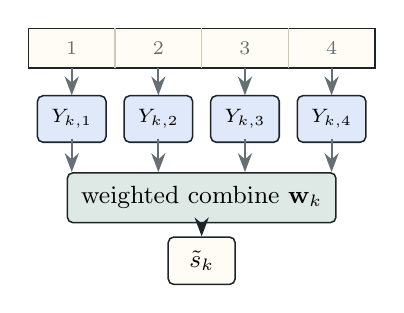
\begin{tikzpicture}[x=1cm,y=1cm,>=Latex]
        % time-sliced symbol bar
        \draw[draw=text,fill=panel,line width=0.55pt] (0,1.30) rectangle (4.4,1.80);
        \foreach \x in {1.10,2.20,3.30} {\draw[draw=grid] (\x,1.30) -- (\x,1.80);}
        \foreach \x/\lab in {0.55/1,1.65/2,2.75/3,3.85/4}
          {\node[font=\scriptsize,text=muted] at (\x,1.55) {\lab};}

        % four aligned partial outputs
        \foreach \x/\lab in {0.55/{Y_{k,1}},1.65/{Y_{k,2}},2.75/{Y_{k,3}},3.85/{Y_{k,4}}} {
          \draw[arrow,draw=muted] (\x,1.30) -- (\x,0.95);
          \node[block,minimum width=0.80cm,minimum height=0.50cm,fill=pilot!15] at (\x,0.65) {\scriptsize $\lab$};
        }

        % combiner
        \node[block,minimum width=1.85cm,minimum height=0.60cm,fill=juna!15] (comb) at (2.20,-0.35)
          {\small weighted combine $\mathbf{w}_k$};
        \foreach \x in {0.55,1.65,2.75,3.85}
          {\draw[arrow,draw=muted] (\x,0.40) -- (comb.north -| {\x,0});}

        % output
        \node[block,minimum width=0.85cm,minimum height=0.50cm,fill=panel] (s) at (2.20,-1.15) {\small $\tilde{s}_k$};
        \draw[arrow] (comb.south) -- (s.north);
      \end{tikzpicture}}
      \vspace{0.05cm}
      \parbox{\linewidth}{\centering\scriptsize Slicing preserves time-variation that a single FFT collapses.}
    \end{column}

    % ---------- Panel 3: who chooses the weights ----------
    \begin{column}{0.28\textwidth}
      \centering
      \textbf{\small 3.\ Who chooses $\mathbf{w}_k$?}\par
      \vspace{0.25cm}
      \resizebox{0.95\linewidth}{!}{%
      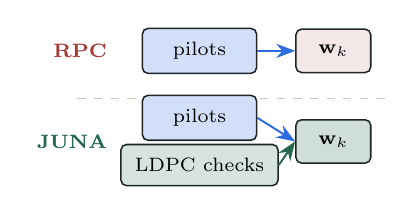
\begin{tikzpicture}[x=1cm,y=1cm,>=Latex]
        % RPC row
        \node[font=\scriptsize\bfseries,text=rpc,anchor=east] at (-0.1,1.15) {RPC};
        \node[block,minimum width=1.45cm,minimum height=0.55cm,fill=pilot!22] (rpil) at (0.95,1.15) {\scriptsize pilots};
        \node[block,minimum width=0.95cm,minimum height=0.55cm,fill=rpc!12] (rw)  at (2.65,1.15) {\scriptsize $\mathbf{w}_k$};
        \draw[arrow,draw=pilot] (rpil.east) -- (rw.west);

        % divider
        \draw[draw=grid,dashed] (-0.6,0.55) -- (3.3,0.55);

        % JUNA row
        \node[font=\scriptsize\bfseries,text=juna,anchor=east] at (-0.1,0.0) {JUNA};
        \node[block,minimum width=1.45cm,minimum height=0.45cm,fill=pilot!22] (jpil)  at (0.95,0.30) {\scriptsize pilots};
        \node[block,minimum width=1.45cm,minimum height=0.45cm,fill=juna!18]  (jcode) at (0.95,-0.30) {\scriptsize LDPC checks};
        \node[block,minimum width=0.95cm,minimum height=0.55cm,fill=juna!22]  (jw)    at (2.65,0.0) {\scriptsize $\mathbf{w}_k$};
        \draw[arrow,draw=pilot] (jpil.east) -- (jw.west);
        \draw[arrow,draw=juna]  (jcode.east) -- (jw.west);
      \end{tikzpicture}}
      \vspace{0.05cm}
      \parbox{\linewidth}{\centering\scriptsize RPC trains $\mathbf{w}_k$ on pilots alone. JUNA adds the LDPC code as a second anchor \textendash{} so far fewer pilots suffice.}
    \end{column}
  \end{columns}
\end{frame}

% =====================================================================
% 8-12. THE FIVE CHANNELS
% =====================================================================
\begin{frame}{Channel A \textendash{} an ``easy'' link (200~m, shallow)}
  \channelimage{figs/profile_095_range200m_bathy30m_tx15m_rx15m_bottom_rigid_surface_windy_bounces_3_fs24000_snr_curve_strict_cpp_yuna_smoothed.png}
  \vspace{0.20cm}
  \begin{columns}[T,onlytextwidth]
    \begin{column}{0.46\textwidth}
      \small\textbf{Setup.} 200~m range, 30~m deep, mild echoes, breezy surface.
    \end{column}
    \begin{column}{0.50\textwidth}
      \small\textbf{Read it.} Without motion, both receivers do fine. With motion, RPC's error rate plateaus much higher; JUNA pushes the floor down. \\\textbf{\color{juna} JUNA delivers $\sim$4$\times$ fewer residual errors.}
    \end{column}
  \end{columns}
\end{frame}

\begin{frame}{Channel B \textendash{} longer range, more selective (400~m)}
  \channelimage{figs/profile_049_range400m_bathy30m_tx15m_rx10m_bottom_pressure_release_surface_rigid_bounces_3_fs24000_snr_curve_strict_cpp_yuna_smoothed.png}
  \vspace{0.20cm}
  \begin{columns}[T,onlytextwidth]
    \begin{column}{0.46\textwidth}
      \small\textbf{Setup.} 400~m range, soft bottom, smoother surface. The channel has deeper notches \textendash{} entire frequencies are nearly silent.
    \end{column}
    \begin{column}{0.50\textwidth}
      \small\textbf{Read it.} Even with strong selectivity, JUNA's use of code structure recovers what pilots alone cannot. \\\textbf{\color{juna} JUNA delivers $\sim$3.8$\times$ fewer residual errors.}
    \end{column}
  \end{columns}
\end{frame}

\begin{frame}{Channel C \textendash{} mid-range with deep notches (500~m)}
  \channelimage{figs/profile_038_range500m_bathy30m_tx15m_rx15m_bottom_pressure_release_surface_windy_bounces_3_fs24000_snr_curve_strict_cpp_yuna_smoothed.png}
  \vspace{0.20cm}
  \begin{columns}[T,onlytextwidth]
    \begin{column}{0.46\textwidth}
      \small\textbf{Setup.} 500~m range, windy surface, soft bottom. Deep frequency notches \textendash{} a harder static channel.
    \end{column}
    \begin{column}{0.50\textwidth}
      \small\textbf{Read it.} The baseline is already working harder. JUNA still extracts a meaningful gain. \\\textbf{\color{juna} JUNA delivers $\sim$3.3$\times$ fewer residual errors.}
    \end{column}
  \end{columns}
\end{frame}

\begin{frame}{Channel D \textendash{} shallow, near-surface ducting (300~m)}
  \channelimage{figs/profile_120_range300m_bathy40m_tx5m_rx5m_bottom_pressure_release_surface_rigid_bounces_3_fs24000_snr_curve_strict_cpp_yuna_smoothed.png}
  \vspace{0.20cm}
  \begin{columns}[T,onlytextwidth]
    \begin{column}{0.46\textwidth}
      \small\textbf{Setup.} 300~m range in 40~m water, both nodes near the surface. Lots of close echoes mixing with motion.
    \end{column}
    \begin{column}{0.50\textwidth}
      \small\textbf{Read it.} The error floor is higher overall \textendash{} this is a genuinely difficult channel. JUNA still helps, but the margin narrows. \\\textbf{\color{juna} JUNA delivers $\sim$1.3$\times$ fewer residual errors.}
    \end{column}
  \end{columns}
\end{frame}

\begin{frame}{Channel E \textendash{} the hard wall (100~m, heavy motion mixing)}
  \channelimage{figs/profile_111_range100m_bathy30m_tx15m_rx10m_bottom_pressure_release_surface_pressure_release_bounces_3_fs24000_snr_curve_strict_cpp_yuna_smoothed.png}
  \vspace{0.20cm}
  \begin{columns}[T,onlytextwidth]
    \begin{column}{0.46\textwidth}
      \small\textbf{Setup.} 100~m range, reflective surface and bottom. Carrier-to-carrier interference dominates.
    \end{column}
    \begin{column}{0.50\textwidth}
      \small\textbf{Read it.} Carrier-to-carrier mixing is so strong that the physics caps what any receiver can do. JUNA matches the baseline here. \\\textbf{\color{muted} JUNA delivers $\sim$1.0$\times$ \textendash{} no harm, no gain.}
    \end{column}
  \end{columns}
\end{frame}

% =====================================================================
% 13. AGGREGATE RESULT
% =====================================================================
\begin{frame}{Across 60 channels: it isn't one lucky example}
  \begin{columns}[T,onlytextwidth]
    \begin{column}{0.58\textwidth}
      \includegraphics[width=\linewidth,height=0.58\paperheight,keepaspectratio]{figs/error_floor_histogram_rpc_yuna_20-120.png}
    \end{column}
    \begin{column}{0.39\textwidth}
      \textbf{What you are seeing}
      \begin{itemize}\setlength{\itemsep}{0.35em}
        \item Each bar counts how many of 60 channels land at a given error rate.
        \item {\color{rpc}\textbf{Red}} = baseline (RPC). {\color{accent}\textbf{Blue}} = JUNA.
        \item JUNA shifts the whole population to the \textbf{left} \textendash{} fewer errors, more often.
      \end{itemize}
      \vspace{0.3em}
      \begin{beamercolorbox}[wd=\linewidth,sep=6pt,rounded=true]{calloutbox}
        \small\textbf{Bottom line:} median residual error drops from $3.0\times10^{-4}$ to $2.0\times10^{-4}$. JUNA helps consistently \textendash{} not just on the easy channels.
      \end{beamercolorbox}
    \end{column}
  \end{columns}
\end{frame}

% =====================================================================
% 14. PILOT RATIO TRADEOFF
% =====================================================================
\begin{frame}{Why JUNA also saves bandwidth}
  \begin{columns}[T,onlytextwidth]
    \begin{column}{0.58\textwidth}
      \includegraphics[width=\linewidth,height=0.55\paperheight,keepaspectratio]{figs/profile020_pilot_ratio_error_floor_stem.png}
    \end{column}
    \begin{column}{0.39\textwidth}
      \textbf{Pilot ratio = overhead.} Pilots are reference notes; the more we add, the less room for payload.
      \vspace{0.5em}

      \begin{itemize}\setlength{\itemsep}{0.3em}
        \item Below $\sim$12\% pilots: nothing works (channel is unidentifiable).
        \item Around 13--15\%: receivers can lock on.
        \item Above 15\%: both flatten \textendash{} but \textbf{JUNA stays lower}.
      \end{itemize}
      \vspace{0.3em}
      \begin{beamercolorbox}[wd=\linewidth,sep=6pt,rounded=true]{calloutbox}
        \small\textbf{Implication:} for the same reliability, JUNA needs fewer pilots \textendash{} that's \textbf{higher useful bit-rate} on the same modem.
      \end{beamercolorbox}
    \end{column}
  \end{columns}
\end{frame}

% =====================================================================
% 15. PROGRESS SO FAR
% =====================================================================
\begin{frame}{Progress at this milestone}
  \begin{columns}[T,onlytextwidth]
    \begin{column}{0.92\textwidth}
      \textbf{Completed}
      \begin{itemize}\setlength{\itemsep}{0.55em}
        \item Formalised why Doppler turns OFDM into a coupled-carrier problem.
        \item Designed JUNA: a joint channel-estimation, symbol-detection, and LDPC-decoding loop.
        \item Validated on a \textbf{60-channel} shallow-water ensemble: consistent error-floor reduction.
        \item Mapped the pilot-ratio tradeoff: JUNA wins more, the leaner the overhead.
      \end{itemize}
    \end{column}
  \end{columns}
  \vspace{0.6cm}
  \begin{center}
    \large\bfseries\color{accent}
    JUNA targets the regime where underwater links have enough signal,\\
    but conventional OFDM loses the message to motion.
  \end{center}
\end{frame}

% =====================================================================
% 17. CLOSING SLIDE
% =====================================================================
\begin{frame}[plain]
  \vspace{0.6cm}
  \begin{center}
    \includegraphics[height=2.4cm,keepaspectratio]{arllogo.png}\\[0.4cm]
    {\Large\bfseries\color{accent} Thank you\par}
    \vspace{0.7cm}
    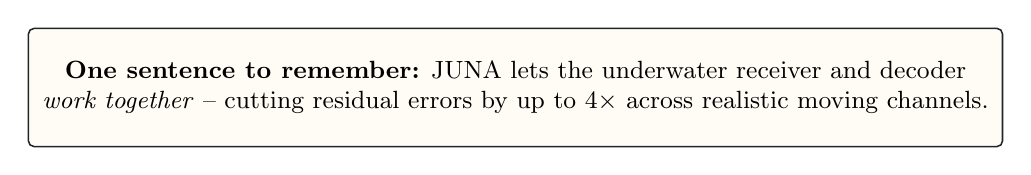
\begin{tikzpicture}
      \node[block,minimum width=11cm,minimum height=1.5cm,fill=panel] (s) {%
        \textbf{One sentence to remember:} JUNA lets the underwater receiver and decoder\\
        \emph{work together} \textendash{} cutting residual errors by up to $4\times$ across realistic moving channels.};
    \end{tikzpicture}
    \vspace{0.7cm}\par
    {\color{muted}\small Questions \textendash{} happy to go deeper on any slide.}
  \end{center}
\end{frame}

% =====================================================================
% BACKUP SLIDES (hidden, available if asked)
% =====================================================================
\appendix

\begin{frame}{Backup \textendash{} anticipated questions}
  \footnotesize
  \begin{columns}[T,onlytextwidth]
    \begin{column}{0.48\textwidth}
      \begin{beamercolorbox}[wd=\linewidth,sep=6pt,rounded=true]{calloutbox}
        \textbf{Q. ``Is this simulated or real?''}\\
        Results so far are simulations using \emph{physically modelled} shallow-water channels (range, depth, bottom type, surface state varied across 60 scenarios). Next step is replay testing with measured channels, then at-sea trials.
      \end{beamercolorbox}
      \vspace{0.3em}
      \begin{beamercolorbox}[wd=\linewidth,sep=6pt,rounded=true]{calloutbox}
        \textbf{Q. ``Hasn't someone solved this already?''}\\
        The conventional fix is more pilots or more complex equalisers. Both cost bandwidth or compute. JUNA reuses work the decoder already does, at modest extra cost.
      \end{beamercolorbox}
      \vspace{0.3em}
      \begin{beamercolorbox}[wd=\linewidth,sep=6pt,rounded=true]{calloutbox}
        \textbf{Q. ``Where does it not help?''}\\
        When carrier-to-carrier mixing is extreme (Channel E), the physics dominates and no receiver wins. JUNA never \emph{hurts}.
      \end{beamercolorbox}
    \end{column}
    \begin{column}{0.48\textwidth}
      \begin{beamercolorbox}[wd=\linewidth,sep=6pt,rounded=true]{calloutbox}
        \textbf{Q. ``What does the user see?''}\\
        Fewer dropped packets, fewer retransmissions, and \textendash{} where engineers want it \textendash{} higher useful data rate at the same reliability.
      \end{beamercolorbox}
      \vspace{0.3em}
      \begin{beamercolorbox}[wd=\linewidth,sep=6pt,rounded=true]{calloutbox}
        \textbf{Q. ``Will this fit on a real modem?''}\\
        Today's prototype is research-grade. A complexity-reduction pass is part of the next phase to bring it inside an embedded modem's budget.
      \end{beamercolorbox}
      \vspace{0.3em}
      \begin{beamercolorbox}[wd=\linewidth,sep=6pt,rounded=true]{calloutbox}
        \textbf{Q. ``How do we know when we've succeeded?''}\\
        Two yardsticks: (i) replay-channel BER matches simulation within tolerance; (ii) at-sea trial shows packet-error-rate reduction at fixed SNR and motion.
      \end{beamercolorbox}
    \end{column}
  \end{columns}
\end{frame}

\end{document}
